\subsection{Performance and mobility, paper \ref{paper:performance_mobility}}
\label{paper:performance_mobility}

\begin{table}[H]
\small
\begin{tabular}{|l|l|l|l|c|} \hline
\textbf{Conference} & \textbf{Date} & \textbf{Loc.} & \textbf{Deadline} & \textbf{Pages} \\ \hline
CloudCom & Dec 15-18 & SG & Jul 31 & 8 \\ \hline
BDCS & Jan 26-27 & SG & Aug 29 & 10	\\ \hline
6th CCW & Dec 8-11 & LDN & Jul 25 & 8 \\ \hline
\end{tabular}
\end{table}

\subsubsection{Abstract}
In an \xcloud topology the resources are dispersed throughout the network. Given that services strictly migrate with the user from, depending on the placement of the service hosts, user mobility will affect the performance perceived performance of the service. The model takes into account the effort of migrating a service and the service performance degradation it introduces.

This paper determines the fundamental service performance issues in system of mobile users with disperead data centres, in relation to the placement of the \xcloud host nodes and explores the user and provider utility of subscribing to an \xcloud node at a certain network depth.

\subsubsection{Related research}
In addition to my first paper we need to find more on 

\subsubsection{Desired model}

\begin{figure}[tb]
	\centering
	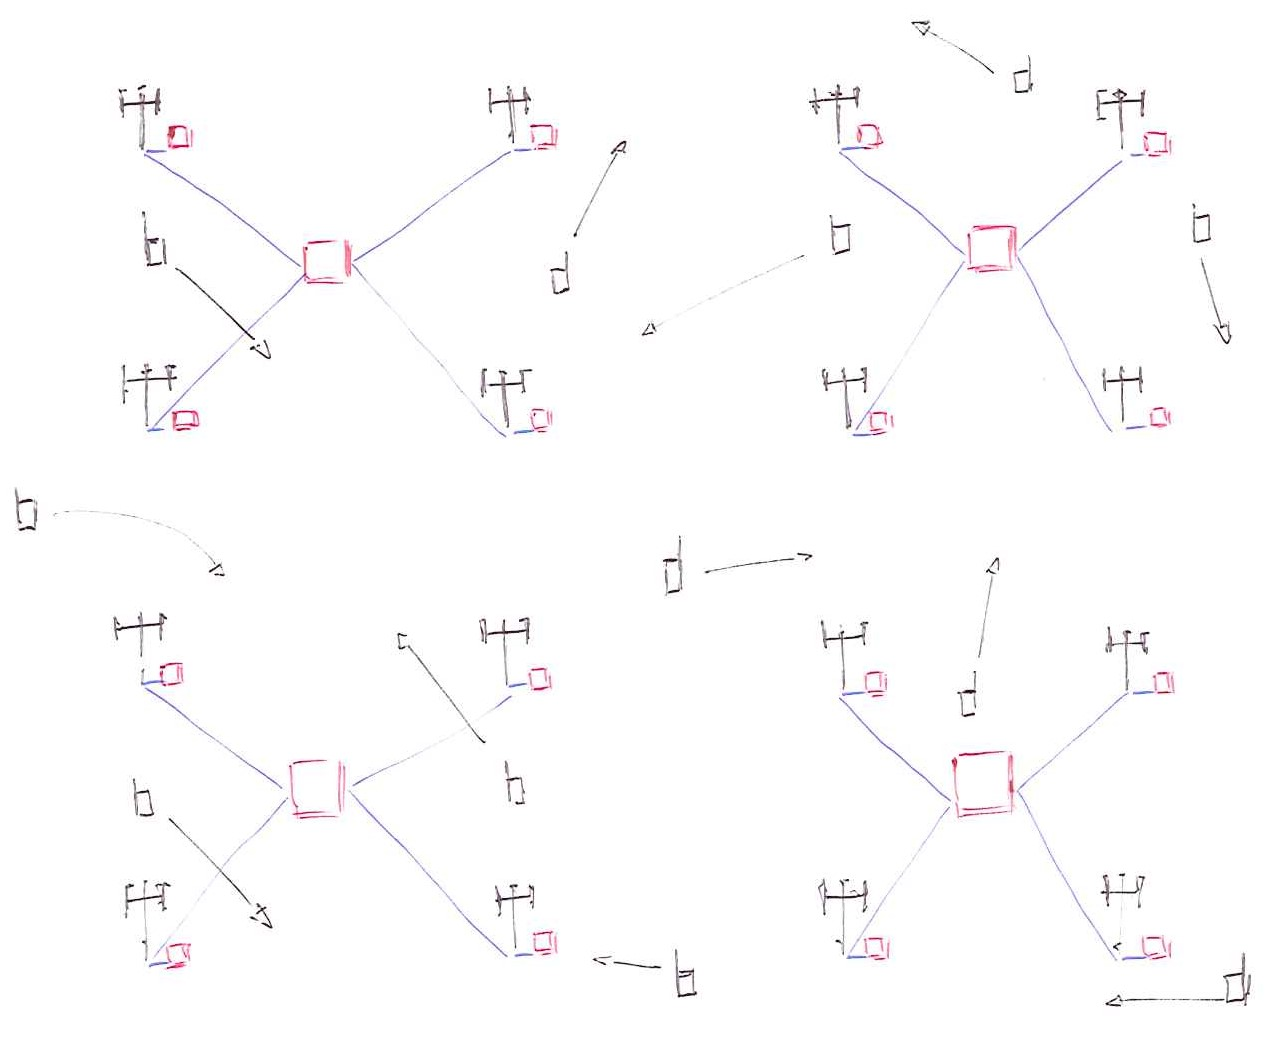
\includegraphics[width=\linewidth]{performance_delay.jpg} 
	\caption{Performance model}
	\label{fig:performance_model}
\end{figure}

As the the topology of the \xcloud and future mobile networks is yet to be determined, and due to the fact that we want to research the effects of mobility without a socio-economic model, the network 

\subsubsection{Simulation}
Multiple runs for each DC/\xcloud placement mode.
\begin{description}
\item[Service]
The traffic generated by and the usage pattern of a simple web application is characteristic of any smaller mobile application. The HTTP traffic model in \cite{liu2001traffic} provides a small scale closed loop traffic model that is representative of light mobile traffic.

\item[Mobility]
The 2 dimensional, multi model, mobility model \cite{bettstetter2001smooth} will provide the uniform mobile network with an relevant distribution of users.

\item[Mobile Access Network] Provided by Williams SIMJava framework. Handover are instantanious and move 

\item[Core network] No delay, no routeing

\item[Server] The server provides VM and DC models that encompass, inucrred VM migration performance degredation in DC and in VM, resulting in a different service time.

Possible service hosting schemes:
\begin{itemize}
\item One service model, one VM is empolyed to host that service for each user.
\item One service model, each VM hosts multiple but each number of users, behaving as multiple services while still being compatible.
\end{itemize}

\end{description}

\subsubsection{Measurements}
At all placement modes:
\begin{itemize}
\item Measure RTT for all packetc at UE
\item Measure DC load
\item Measure ratio of requests generated vs. processed in \xcloud node
\item Identify the incurred VM migration load
\end{itemize}

\subsubsection{Future research}
\begin{itemize}
\item Optimal service/VM migration/placement in relevant topology
\item Performance in LTE newtork topology using LTE-SIM \cite{5634134}
\end{itemize}